%This is the third chapter of the dissertation

%The following command starts your chapter. If you want different titles used in your ToC and at the top of the page throughout the chapter, you can specify those values here. Since Columbia doesn't want extra information in the headers and footers, the "Top of Page Title" value won't actually appear.

\pagestyle{cu}
\graphicspath{{./Chapter3/Figures/}}
\chapter[Table of Contents Title][Top of Page Title]{Title of Chapter 3}

Here you can write some introductory remarks about your chapter.
I like to give each sentence its own line.

When you need a new paragraph, just skip an extra line.

\section*{New Section}

By using the asterisk to start a new section, I keep the section from appearing in the table of contents.
If you want your sections to be numbered and to appear in the table of contents, remove the asterisk.

\begin{figure}
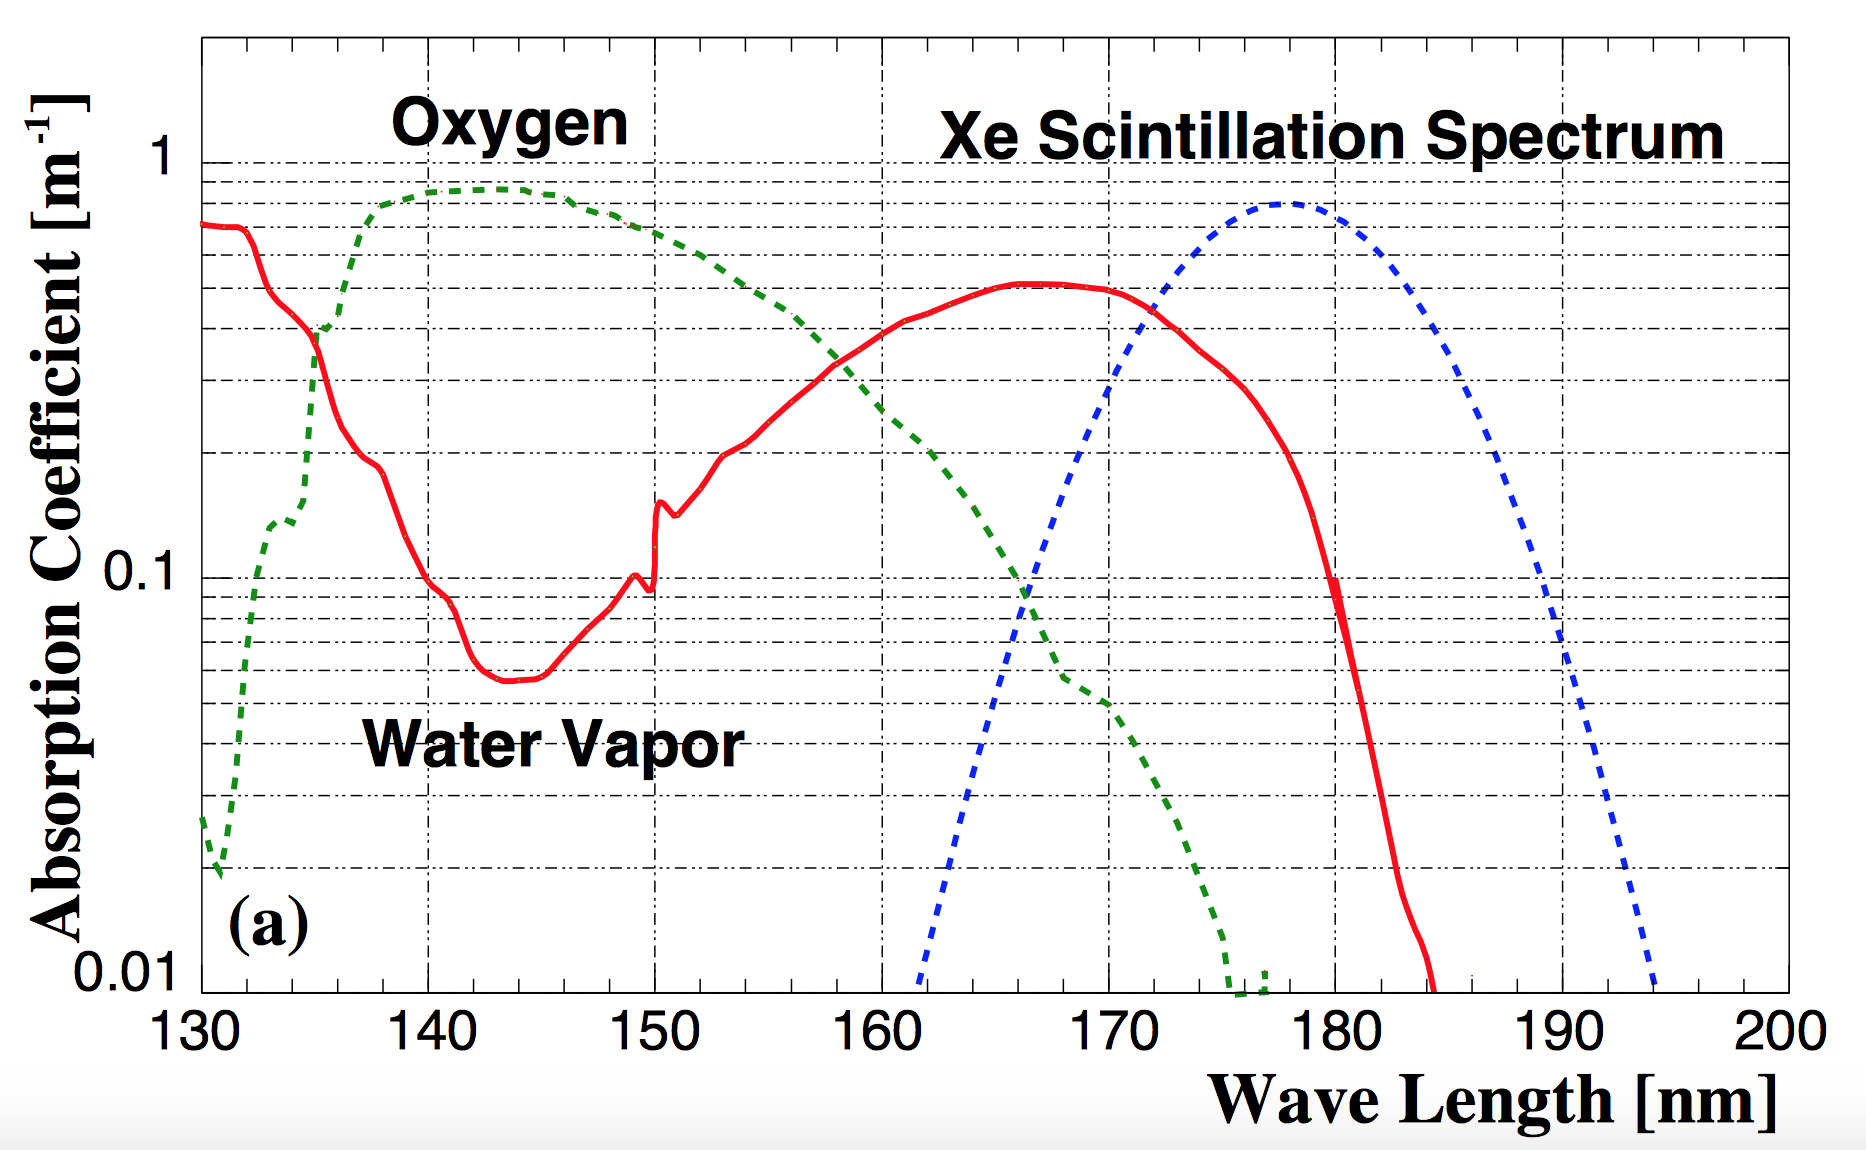
\includegraphics[\width=0.8\textwidth]{AbsorptionSpectra}
\caption{\citeref{Ozone2005}}
\end{figure}